\documentclass{beamer}

\usepackage{comment}
\usepackage{color}
\usepackage{listings}
\usepackage{verbatim}
\usepackage{multicol}
\usepackage{booktabs}
\definecolor{green}{RGB}{0,128,0}

\newcommand\gehcomment[1]{{{\color{orange} #1}}}
\newcommand\add[1]{{{\color{blue} #1}}}
\newcommand\remove[1]{\sout{{\color{red} #1}}}
\newcommand\codecomment[1]{{{\color{green} #1}}}
\newcommand\redcomment[1]{{{\color{red} #1}}}
\newcommand\bluecomment[1]{{{\color{blue} #1}}}
\newcommand\greencomment[1]{{{\color{green} #1}}}
\newcommand\magentacomment[1]{{{\color{magenta} #1}}}

\begin{comment}
\tiny
\scriptsize
\footnotesize
\small
\normalsize
\large
\Large
\LARGE
\huge
\Huge
\end{comment}

\begin{document}
\title{Multiphase - Gas Injection}
\author{Emily Stein}
\date{\today}

%\frame{\titlepage}

%-----------------------------------------------------------------------------
\section{Location of Example}

\begin{frame}[fragile,containsverbatim]\frametitle{Location}

Location of this example problem:

\begin{semiverbatim}
> cd \$PFLOTRAN_DIR
> cd shortcourse/exercises/heater
> ls

heater.in
heater.py
heater_usg.h5
sideset_0.ss
\end{semiverbatim}

\end{frame}

%-----------------------------------------------------------------------------
\subsection{Command Line}
\begin{frame}[fragile]\frametitle{Command Line}
This problem might take a few minutes, so let's begin the simulation now.

\begin{itemize}
  \item Run the simulation
\end{itemize}

\begin{semiverbatim}
> cd \$PFLOTRAN_DIR
> cd shortcourse/exercises/heater
> pflotran -input_prefix heater
\end{semiverbatim}

\end{frame}

%-----------------------------------------------------------------------------
\section{Description of Heater}

\subsection{Heater Conceptual Model}

\begin{frame}\frametitle{Description of Heater Scenario}
The ``Heater Scenario'' demonstrates how to set up a multiphase flow simulation using \redcomment{GENERAL MODE}. It simulates a heat source (such as radioactive waste) in a partially saturated domain. It also demonstrates use of an \redcomment{unstructured grid}. Assumptions include:
\begin{itemize}
  \item Problem domain: $15 \times 1 \times 30$ m (x $\times$ y $\times$ z)
  \item Grid resolution: Varies in an unstructured grid
  \item Flow mode: General
  \item Heat Source: Rate scaled by cell volume
  \item Maximum time step size: changes with simulation time
  \item Total simulation time: 100 y
\end{itemize}

\end{frame}

%-----------------------------------------------------------------------------
\frame{\frametitle{2D Heater Scenario Schematic}
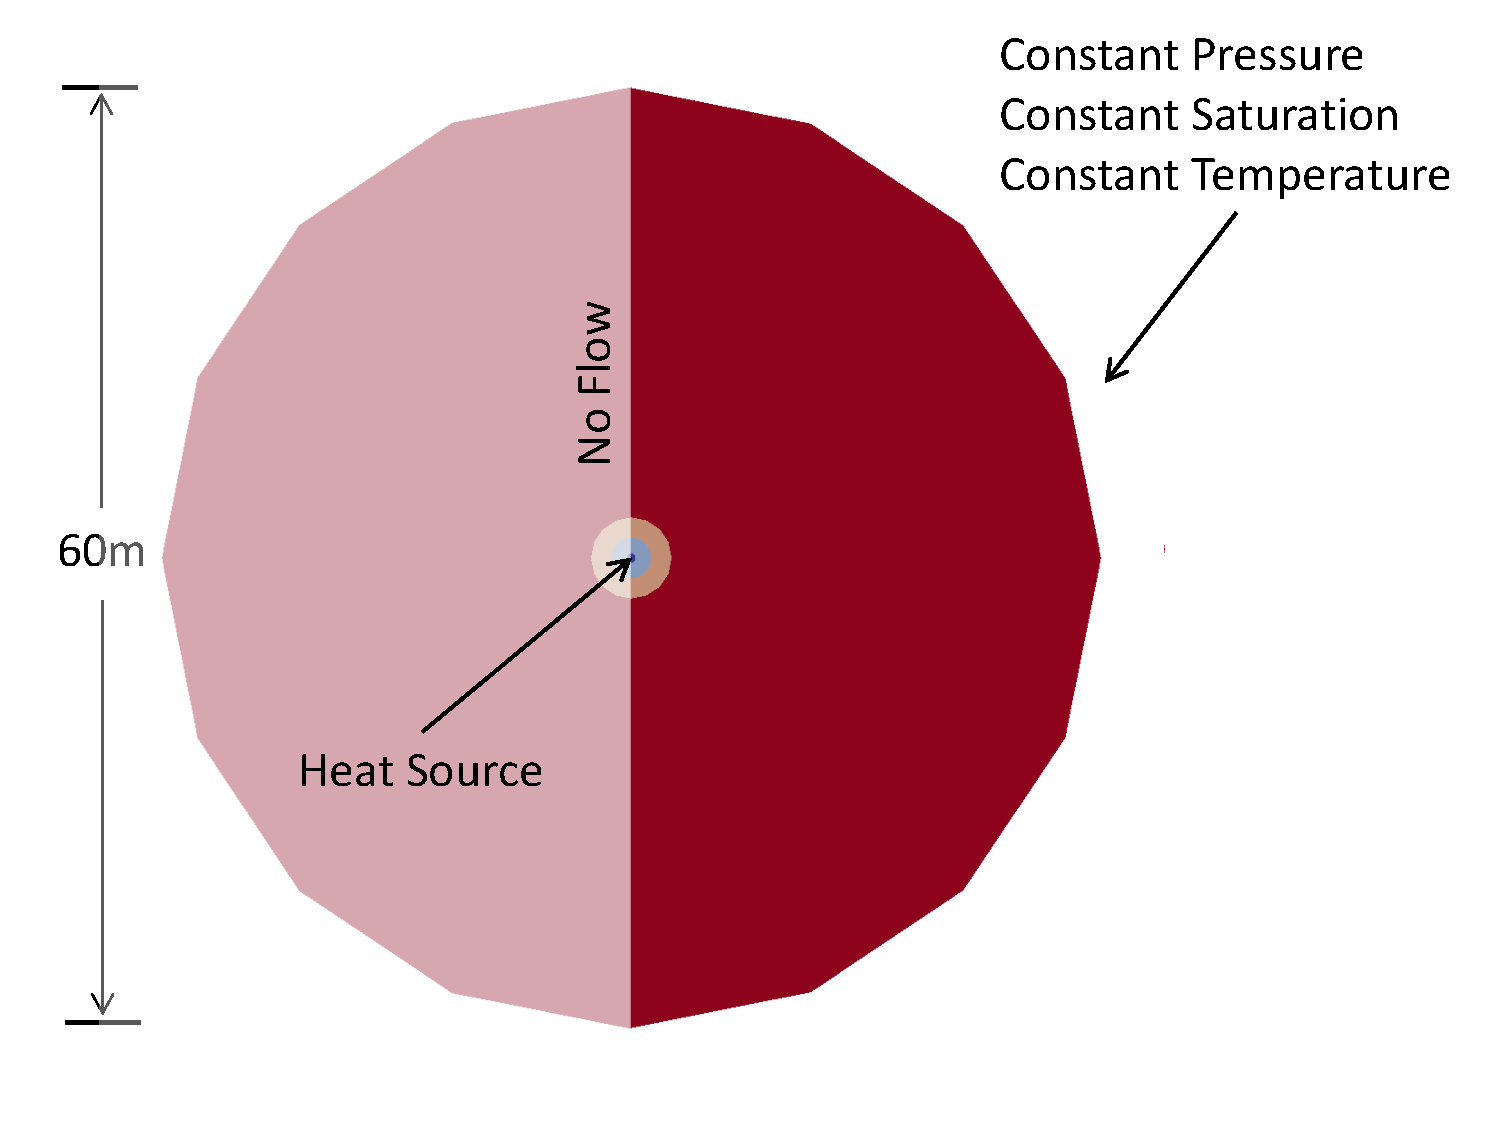
\includegraphics[width=\linewidth]{./heater_bc}
}

%-----------------------------------------------------------------------------
\frame{\frametitle{2D Heater Initial Conditions}
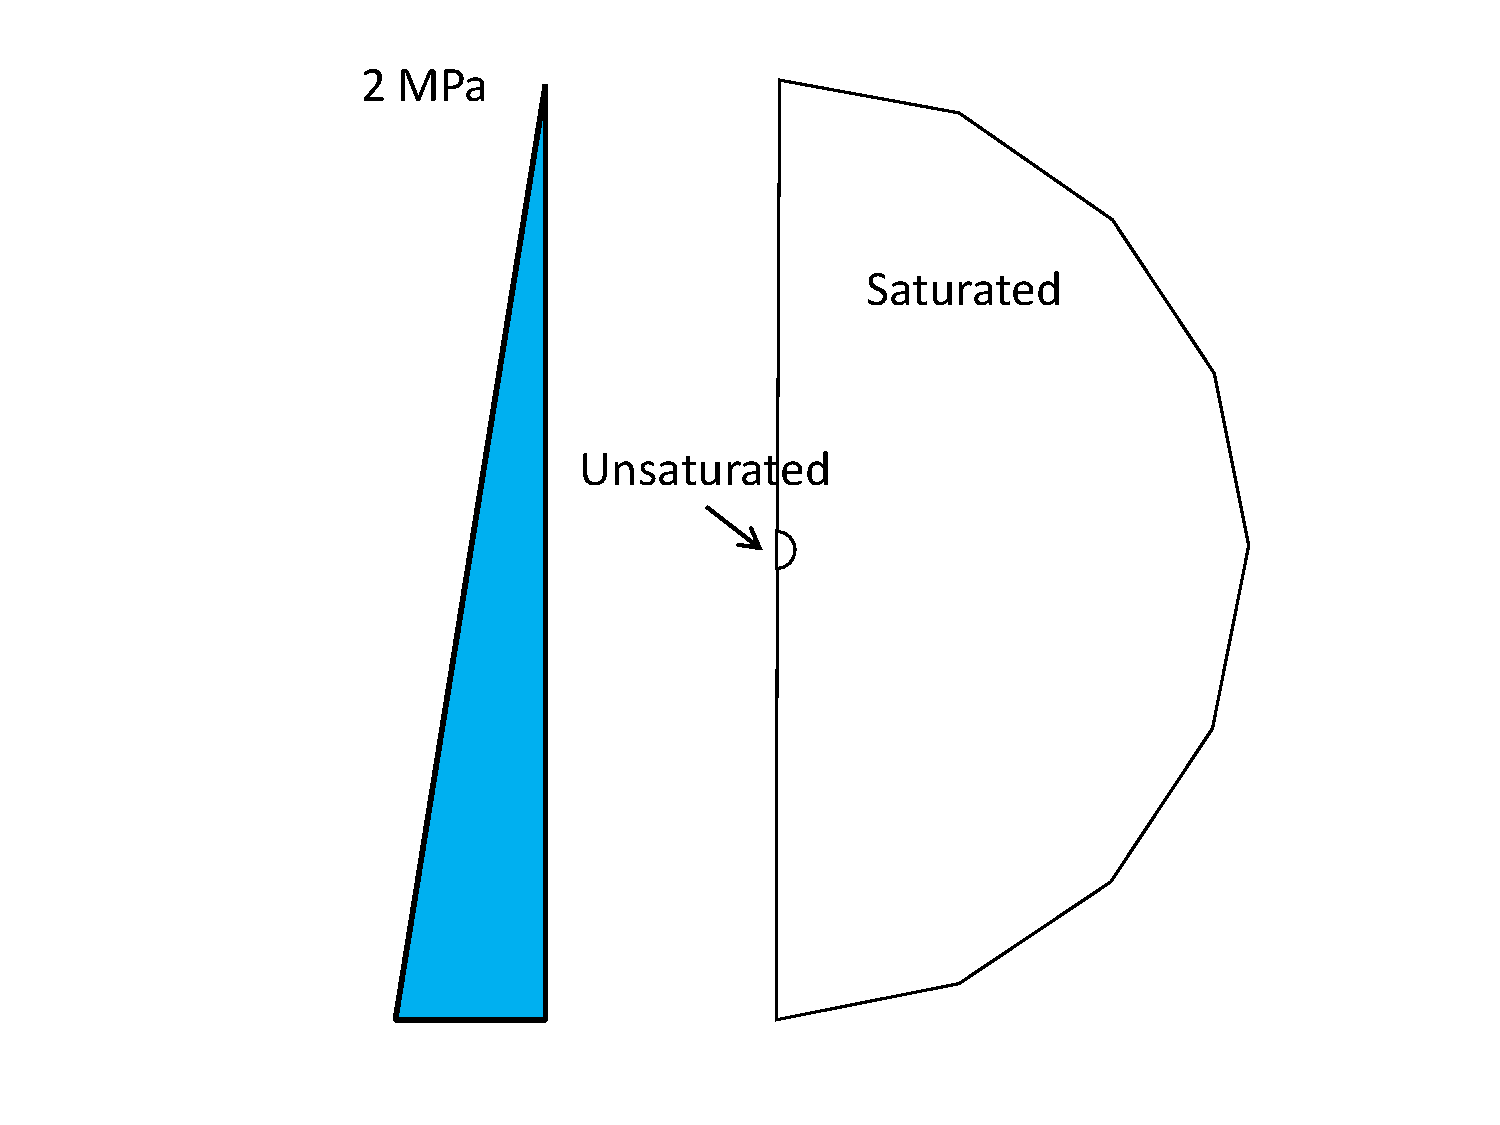
\includegraphics[width=\linewidth]{./heater_ic}
}

%-----------------------------------------------------------------------------
\frame{\frametitle{2D Heater Mesh File}
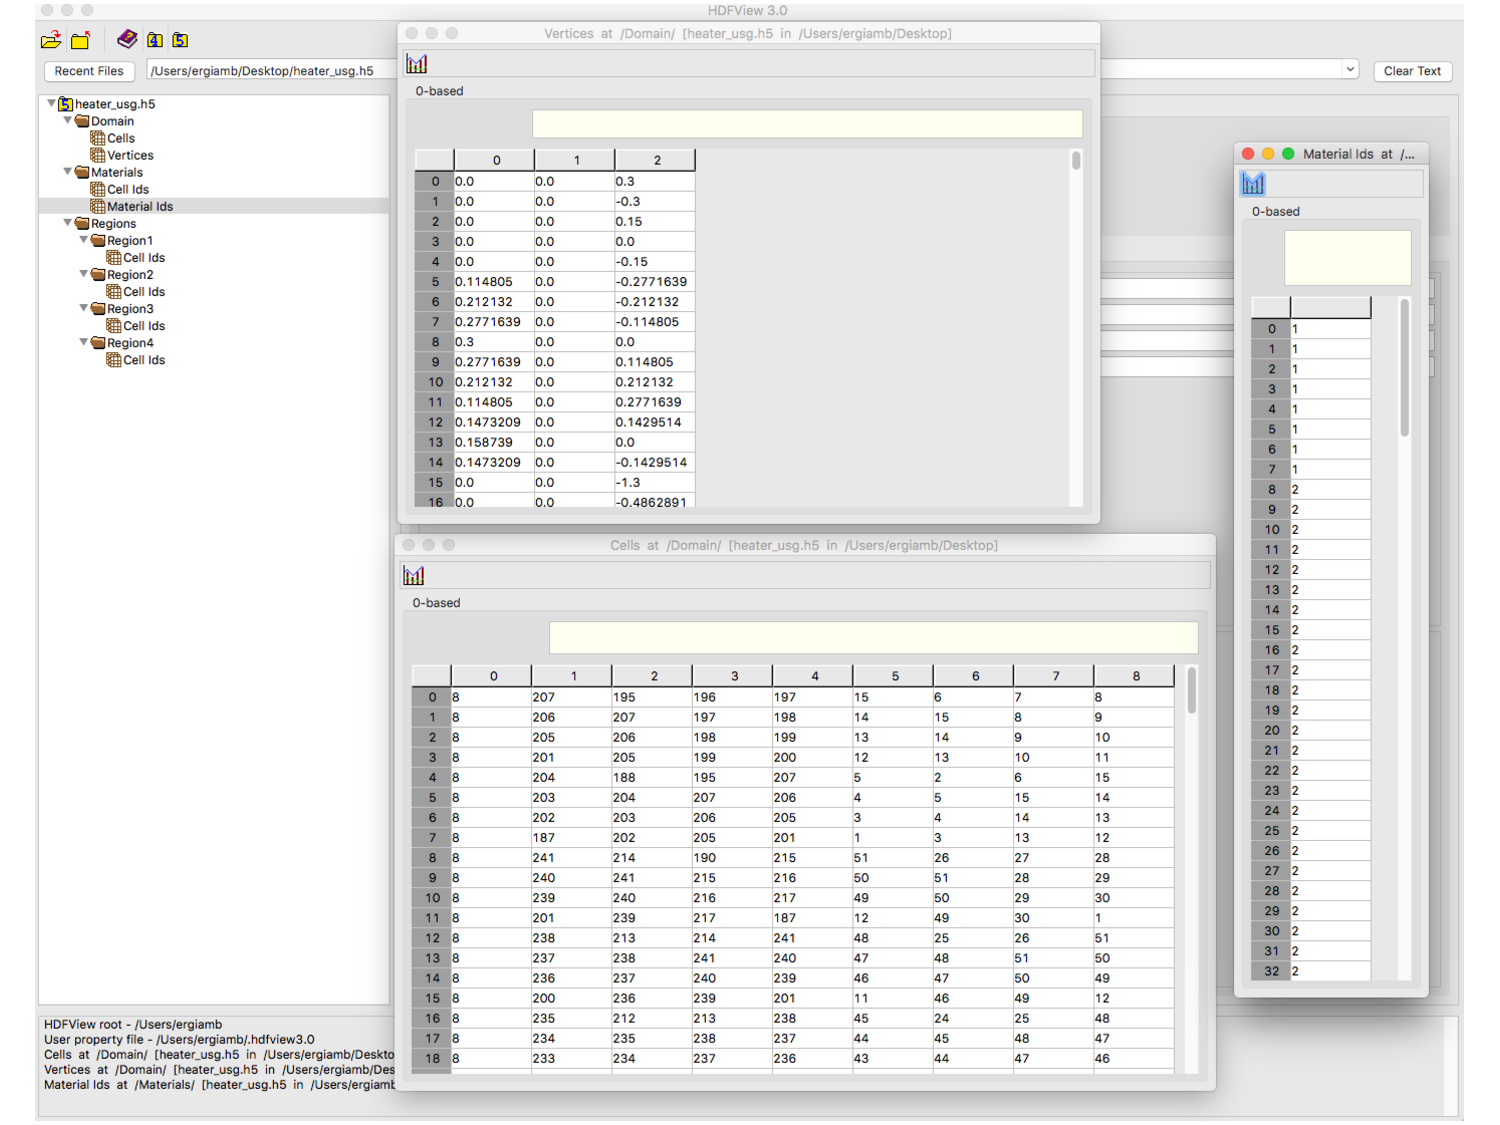
\includegraphics[width=\linewidth]{./heater_hdfview}
}

%-----------------------------------------------------------------------------
\section{Description of Input Deck}

%-----------------------------------------------------------------------------
\subsection{SIMULATION}

\begin{frame}[fragile]\frametitle{SIMULATION}

\begin{itemize}
  \item Multiphase flow (\redcomment{General mode})
  \item with \redcomment{options}
\end{itemize}

\begin{semiverbatim}\small
SIMULATION
  SIMULATION_TYPE SUBSURFACE
  PROCESS_MODELS
    SUBSURFACE_FLOW flow
      MODE GENERAL \bluecomment{! two-phase flow and energy}
      OPTIONS
        ANALYTICAL_DERIVATIVES
      /   
    /   
  /
END

SUBSURFACE
...
END_SUBSURFACE
\end{semiverbatim}

\end{frame}

%-----------------------------------------------------------------------------
\subsection{GRID}

\begin{frame}[fragile]\frametitle{GRID}

\begin{itemize}
  \item Implicit \redcomment{unstructured} grid 
\end{itemize}

\begin{semiverbatim}
GRID
  TYPE UNSTRUCTURED ./heater_usg.h5
END
\end{semiverbatim}

\end{frame}

%-----------------------------------------------------------------------------
\subsection{FLUID\_PROPERTY}

\begin{frame}[fragile]\frametitle{FLUID\_PROPERTY}
\begin{itemize}
  \item Diffusion of dissolved gas in \redcomment{liquid phase}
  \item Diffusion of water vapor in \redcomment{gas phase}
\end{itemize}

\begin{semiverbatim}

FLUID_PROPERTY
  PHASE LIQUID \bluecomment{! for diffusion of dissolved gas}
  DIFFUSION_COEFFICIENT 1.d-9
END

FLUID_PROPERTY
  PHASE GAS \bluecomment{! for diffusion of water vapor}
  DIFFUSION_COEFFICIENT 2.1d-5
END
\end{semiverbatim}

\end{frame}

%-----------------------------------------------------------------------------
\subsection{OUTPUT}

\begin{frame}[fragile]\frametitle{OUTPUT}
\begin{itemize}
  \item Print a \redcomment{snapshot} of entire solution periodically
  \item Print the solution at \redcomment{observation points} every time step
  \item Print \redcomment{mass balance} file every time step
  \item Choose output \redcomment{variables}
\end{itemize}

\end{frame}

\begin{frame}[fragile]\frametitle{OUTPUT}

\begin{semiverbatim}\small
OUTPUT
  SNAPSHOT_FILE
    FORMAT HDF5
    PERIODIC TIME 1. d between 0. d and 10. d  \bluecomment{! every 1 day}
    PERIODIC TIME 10. d between 0. d and 300. d  \bluecomment{! every 10 days}
    PERIODIC TIME 1. y between 0. y and 10. y \bluecomment{! every 1 year}
    PERIODIC TIME 10. y between 0. y and 100. y \bluecomment{! etc.}
  /
  OBSERVATION_FILE
    PERIODIC TIMESTEP 1 \bluecomment{! print every time step}
  /
  MASS_BALANCE_FILE
    PERIODIC TIMESTEP 1 \bluecomment{! print every time step}
  /
  VELOCITY_AT_CENTER    \bluecomment{! of cell}
  VARIABLES
    TEMPERATURE
    LIQUID_SATURATION   \bluecomment{! see input deck for more}
  /
END
\end{semiverbatim}

\end{frame}

%-----------------------------------------------------------------------------
\subsection{TIME}

\begin{frame}[fragile]\frametitle{TIME}
\begin{itemize}
  \item \redcomment{Final} simulation \redcomment{time} = 100 y
  \item \redcomment{Maximum time step size} = 10 y
\end{itemize}

\begin{semiverbatim}

TIME
  FINAL_TIME 100.d0 y \bluecomment{! end of simulation}
  MAXIMUM_TIMESTEP_SIZE .1 d at 0. d \bluecomment{! start small}
  MAXIMUM_TIMESTEP_SIZE 1. d at 1. d \bluecomment{! allow larger}
  MAXIMUM_TIMESTEP_SIZE 10. d at 10. d \bluecomment{! at late times}
  MAXIMUM_TIMESTEP_SIZE 1. y at 1. y
  MAXIMUM_TIMESTEP_SIZE 10. y at 10. y
END
\end{semiverbatim}

\end{frame}

%-----------------------------------------------------------------------------
\subsection{MATERIAL\_PROPERTY}

\begin{frame}[fragile]\frametitle{MATERIAL\_PROPERTY}
\begin{itemize}
  \item Energy equations require:
  \begin{itemize}
    \item \redcomment{mineral density}
    \item \redcomment{thermal conductivity} (bulk wet and dry)
    \item \redcomment{mineral heat capacity}
  \end{itemize}
\end{itemize}

\begin{semiverbatim}\small
MATERIAL_PROPERTY shale \bluecomment{! define material} \greencomment{shale}
  ID 4
  CHARACTERISTIC_CURVES default
  POROSITY 0.20
  TORTUOSITY 0.11
  ROCK_DENSITY 2700. \bluecomment{! density of the solid phase}
  THERMAL_CONDUCTIVITY_DRY 1.0d0 \bluecomment{! dry bulk medium}
  THERMAL_CONDUCTIVITY_WET 1.7d0 \bluecomment{! wet bulk medium}
  HEAT_CAPACITY 830. \bluecomment{! heat capacity of the solid phase}
  PERMEABILITY
    PERM_ISO 1.d-19
  /
END
\end{semiverbatim}
\end{frame}

\begin{frame}[fragile]\frametitle{MATERIAL\_PROPERTY}
\begin{semiverbatim}
MATERIAL_PROPERTY drz \bluecomment{!} \greencomment{drz} \bluecomment{= disturbed rock zone}
  ID 3
  CHARACTERISTIC_CURVES default
  POROSITY 0.20
  TORTUOSITY 0.11
  ROCK_DENSITY 2700. \bluecomment{! kg/m3}
  THERMAL_CONDUCTIVITY_DRY 1.0d0 \bluecomment{! W/(m-K)}
  THERMAL_CONDUCTIVITY_WET 1.7d0 \bluecomment{! W/(m-K)}
  HEAT_CAPACITY 830. \bluecomment{! J/(kg-K)}
  PERMEABILITY
    PERM_ISO 1.d-18
  /
END
\end{semiverbatim}
\end{frame}

\begin{frame}[fragile]\frametitle{MATERIAL\_PROPERTY}
\begin{semiverbatim}
MATERIAL_PROPERTY buffer \bluecomment{! define material} \greencomment{buffer}
  ID 2
  CHARACTERISTIC_CURVES default
  POROSITY 0.35
  TORTUOSITY 0.23
  ROCK_DENSITY 2700. \bluecomment{! kg/m3}
  THERMAL_CONDUCTIVITY_DRY 0.6d0 \bluecomment{! W/(m-K)}
  THERMAL_CONDUCTIVITY_WET 1.2d0 \bluecomment{! W/(m-K)}
  HEAT_CAPACITY 830. \bluecomment{! J/(kg-K)}
  PERMEABILITY
    PERM_ISO 1.d-20
  /
END
\end{semiverbatim}
\end{frame}

\begin{frame}[fragile]\frametitle{MATERIAL\_PROPERTY}
\begin{semiverbatim}
MATERIAL_PROPERTY heater \bluecomment{! define material} \greencomment{heater}
  ID 1
  CHARACTERISTIC_CURVES default
  POROSITY 0.01 \bluecomment{! a small value}
  TORTUOSITY 1.0
  ROCK_DENSITY 5000. \bluecomment{! thermally this is stainless steel}
  THERMAL_CONDUCTIVITY_DRY 16.7d0 
  THERMAL_CONDUCTIVITY_WET 16.7d0 
  HEAT_CAPACITY 466. 
  PERMEABILITY
    PERM_ISO 1.d-20 \bluecomment{! same as buffer}
  /
END
\end{semiverbatim}
\end{frame}
%-----------------------------------------------------------------------------
\subsection{CHARACTERISTIC\_CURVES}

\begin{frame}[fragile,containsverbatim]\frametitle{CHARACTERISTIC\_CURVES}
\begin{itemize}\small
  \item Van Genuchten \redcomment{saturation function}
  \item Mualem \redcomment{relative permeability} for liquid and gas phases
  \item Use \greencomment{default} with all materials to make problem run faster
\end{itemize}
\begin{semiverbatim}\small
CHARACTERISTIC_CURVES default \bluecomment{! define} \greencomment{default}
  SATURATION_FUNCTION VAN_GENUCHTEN
    ALPHA 1.d-4
    M 0.5
    LIQUID_RESIDUAL_SATURATION 0.1d0
  /
  PERMEABILITY_FUNCTION MUALEM_VG_LIQ
    PHASE LIQUID
    M 0.5
    LIQUID_RESIDUAL_SATURATION 0.1d0
  /
  PERMEABILITY_FUNCTION MUALEM_VG_GAS
    PHASE GAS
    M 0.5
    LIQUID_RESIDUAL_SATURATION 0.1d0
    GAS_RESIDUAL_SATURATION 0.1d0
  /
END
\end{semiverbatim}
\end{frame}

%-----------------------------------------------------------------------------
\subsection{REGION}

\begin{frame}[fragile]\frametitle{REGION}
Regions will be used for:
\begin{itemize}\small
  \item{assignment of \redcomment{IC} and \redcomment{BC}}
  \item{location of heat \redcomment{source}}
\end{itemize}

\begin{semiverbatim}\small
REGION all               \bluecomment{! define region:} \greencomment{all}
  COORDINATES            \bluecomment{! using coordinates}
    -1.d20 -1.d20 -1.d20 \bluecomment{! very large volume}
     1.d20  1.d20  1.d20 \bluecomment{! nothing will be left out}
  /
END
\bluecomment{! heater and buffer}
REGION Region1 \bluecomment{! read} \greencomment{Region1} \bluecomment{(heater)from file}
  FILE ./heater_usg.h5
END
REGION Region2 \bluecomment{! read} \greencomment{Region1} \bluecomment{(buffer) from file}
  FILE ./heater_usg.h5
END
\bluecomment{! faces for DIRICHLET BC}
REGION outer_face \bluecomment{! read} \greencomment{outer_face} \bluecomment{from file}
  FILE ./sideset_0.ss
END
\end{semiverbatim}
\end{frame}
%-----------------------------------------------------------------------------
\subsection{OBSERVATION}

\begin{frame}[fragile]\frametitle{OBSERVATION}
\begin{itemize}
  \item{Define three more regions for \redcomment{output}}
\end{itemize}

\begin{semiverbatim}\small
REGION buffer_obs1 \bluecomment{! define region:} \greencomment{buffer_obs1}
  COORDINATE .4d0 0.5d0 0.1d0 \bluecomment{! note single coordinate}
END

REGION buffer_obs2 \bluecomment{! define region:} \greencomment{buffer_obs2}
  COORDINATE .6d0 0.5d0 0.1d0
END

REGION buffer_obs3 \bluecomment{! define region:} \greencomment{buffer_obs3}
  COORDINATE .8d0 0.5d0 0.1d0
END
\end{semiverbatim}
\end{frame}

\begin{frame}[fragile]\frametitle{OBSERVATION}
\begin{itemize}
  \item{Use regions as observation points}
\end{itemize}

\begin{semiverbatim}\small
OBSERVATION
  REGION buffer_obs1 \bluecomment{! use} \greencomment{buffer_obs1} \bluecomment{as obs pt}
END

OBSERVATION
  REGION buffer_obs2 \bluecomment{! use} \greencomment{buffer_obs2} \bluecomment{as obs pt}
END

OBSERVATION
  REGION buffer_obs3 \bluecomment{! use} \greencomment{buffer_obs3} \bluecomment{as obs pt}
END
\end{semiverbatim}
\end{frame}

%-----------------------------------------------------------------------------
\subsection{FLOW\_CONDITION}

\begin{frame}[fragile]\frametitle{FLOW\_CONDITION}
\begin{itemize}
  \item{Single phase liquid, hydrostatic}
  \item{Use for \redcomment{IC} and \redcomment{BC}}
\end{itemize}

\begin{semiverbatim}
FLOW_CONDITION initial_shale \bluecomment{! define} \greencomment{initial_shale}
  TYPE
    LIQUID_PRESSURE HYDROSTATIC
    MOLE_FRACTION DIRICHLET
    TEMPERATURE DIRICHLET
  /
  DATUM 0.d0 0.d0 0.d0 \bluecomment{! center of drift}
  LIQUID_PRESSURE 2.d6 \bluecomment{! Pa}
  MOLE_FRACTION 1.d-8  \bluecomment{! dissolved gas}
  TEMPERATURE 25.d0    \bluecomment{! degrees C}
END
\end{semiverbatim}
\end{frame}

\begin{frame}[fragile]\frametitle{FLOW\_CONDITION}
\begin{itemize}
  \item{Two-phase liquid and gas}
  \item{Use for \redcomment{IC}}
\end{itemize}

\begin{semiverbatim}
FLOW_CONDITION initial_buffer \bluecomment{! define} \greencomment{initial_buffer}
  TYPE
    GAS_PRESSURE DIRICHLET
    GAS_SATURATION DIRICHLET
    TEMPERATURE DIRICHLET
  /
  GAS_PRESSURE 101325.d0 \bluecomment{! Pa (atmospheric)}
  GAS_SATURATION 0.8d0
  TEMPERATURE 25.d0      \bluecomment{! degrees C}
END
\end{semiverbatim}
\end{frame}

\begin{frame}[fragile]\frametitle{FLOW\_CONDITION}
\begin{itemize}
  \item{\redcomment{Source} term}
  \item{Use for waste package heat}
\end{itemize}

\begin{semiverbatim}
FLOW_CONDITION heater \bluecomment{! define} \greencomment{heater}
  TYPE
    RATE SCALED_MASS_RATE VOLUME \bluecomment{! volume averaged}
  /
  SYNC_TIMESTEP_WITH_UPDATE
  RATE LIST
    TIME_UNITS d
    DATA_UNITS kg/s kg/s W
    \bluecomment{! time liquid gas energy}
     0.0d0 0.d0 0.d0   0.d0
     0.1d0 0.d0 0.d0 150.d0
    365.d0 0.d0 0.d0   0.d0
  /
END
\end{semiverbatim}
\end{frame}

%-----------------------------------------------------------------------------
\subsection{Couplers}

\begin{frame}[fragile]\frametitle{Couplers}

\begin{itemize}
  \item \redcomment{Initial condition}: flow condition \greencomment{initial\_shale} with region \greencomment{all}
  \item \redcomment{Initial condition}: flow condition \greencomment{initial\_buffer} with \greencomment{Region1} and \greencomment{Region2}
\end{itemize}

\begin{semiverbatim}\small
\bluecomment{! saturated initial condition}
INITIAL_CONDITION shale \bluecomment{! optional name}
  FLOW_CONDITION initial_shale
  REGION all
END
\bluecomment{! two-phase initial condition}
INITIAL_CONDITION heater \bluecomment{! optional name}
  FLOW_CONDITION initial_buffer
  REGION Region1
END
\bluecomment{! two-phase initial condition}
INITIAL_CONDITION buffer \bluecomment{! optional name}
  FLOW_CONDITION initial_buffer
  REGION Region2
END
\end{semiverbatim}
\end{frame}

\begin{frame}[fragile]\frametitle{Couplers}

\begin{itemize}
  \item \redcomment{Boundary condition}: flow condition \greencomment{initial\_shale} with region \greencomment{outer\_face}
  \item \redcomment{Source}: flow condition \greencomment{heatsource} with region \greencomment{Region1}
\end{itemize}

\begin{semiverbatim}\small
\bluecomment{! boundary conditions}
BOUNDARY_CONDITION open \bluecomment{! optional name}
  FLOW_CONDITION initial_shale
  REGION outer_face
END

\bluecomment{! source_sink }
SOURCE_SINK heat \bluecomment{! optional name}
  FLOW_CONDITION heatsource
  REGION Region1
END
\end{semiverbatim}
\end{frame}

\begin{frame}[fragile]\frametitle{Couplers}
\begin{itemize}
  \item{Material property IDs for each cell are read from an h5 file}
\end{itemize}

\begin{semiverbatim}
STRATA \bluecomment{! Materials from file}
  FILE ./heater_usg.h5
END
\end{semiverbatim}
\end{frame}

%-----------------------------------------------------------------------------
\subsection{END\_SUBSURFACE}
\begin{frame}[fragile]\frametitle{END\_SUBSURFACE}

\begin{itemize}
  \item Close the SUBSURFACE block
\end{itemize}

\begin{semiverbatim}
END_SUBSURFACE \bluecomment{! That's all!}
\end{semiverbatim}
\end{frame}

%-----------------------------------------------------------------------------
\subsection{Command Line}
\begin{frame}[fragile]\frametitle{Command Line}

\begin{itemize}
  \item Plot the results
\end{itemize}

\begin{semiverbatim}
> python heater.py
\end{semiverbatim}

\end{frame}

%-----------------------------------------------------------------------------
\end{document}
